\section{Introduction}
\label{sec:intro}
%
Mobile manipulation is the field of robotics concerned with highly capable robots 
characterized by their locomotion and manipulation ability. Such robots
are getting ever more attention as they will be deployed to human-shared environments, 
like households or warehouses. In such dynamic environments, fast trajectory generation
is crucial to avoid collisions and react quickly to changing goal definitions. 

Trajectory generation is often addressed by solving an optimization problem
that consists of a scalar objective function -- the dynamics or transition
function -- and several constraints. As the degrees of freedom and number of
constraints increase, solving that problem in real-time becomes challenging.
This is especially limiting in the case of mobile manipulation
\cite{spahn2021coupled}. Optimization fabrics represent a different approach to
the problem, as they formulate trajectory generation as the
shortest-geodesic-problem in a manifold of the configuration space
\cite{Karaman2011}. 

With optimization fabrics, different components, or desired behaviors, such as
collision avoidance and joint limit avoidance, are combined using Riemannian
metrics. As the structure of the resulting trajectory generation methods
remains unchanged across all time steps, it can be composed before runtime,
thus saving computational costs during executing. 
Optimization fabrics, but also their predecessor Riemannian Motion Policies
(RMPs), have shown impressive results for several manipulator applications,
including dynamic and crowded environments \cite{Wyk2022,Xie2021,Spahn2022}.
However, despite their theoretical properties of inherent collision avoidance
and convergence, these methods require expertise and intuition to tune
individual components to generate smooth and well-behaving trajectories. 
%
\begin{figure}
    \centering
    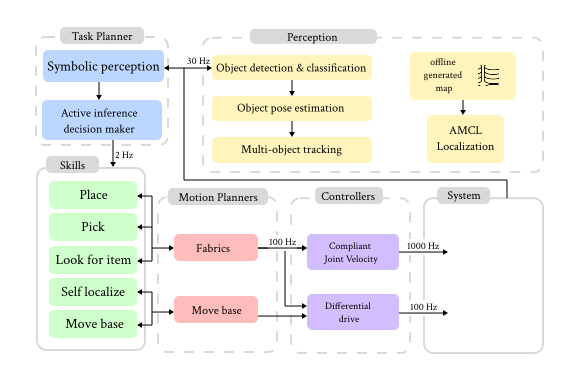
\includegraphics[width=0.8\linewidth]{overview}
    \captionsetup{belowskip=-20pt}
    \caption{
      Overview of one trial in the tuning pipeline for symbolic optimization
      fabrics. The objective function is evaluated after an entire trial run is
      simulated. Using Bayesian optimization, a new parameter set is suggested
      based on the history of trials. The best parameter set is extracted from
      all trials.
    }
    \label{fig:overview}
\end{figure}
%

\textit{Contributions:}
To address this issue, we formulate optimization fabrics as a \textbf{symbolic
trajectory generation} method. Precisely, the combination of the individual
components (joint limit avoidance, goal reaching, collision avoidance, etc.) is
performed in a parameterized way before runtime. Separating composition and
evaluation allows for changing the individual parameters at runtime while
achieving low computational costs. Additionally, this allows formulating
parameter-tuning as a constrained optimization problem. Solving this problem
effectively \textbf{automates the tuning process} systematically using
Bayesian optimization. We show that automated tuning requires only few trials
to achieve similar performance to an expert in the field, and systematically
outperforms a randomized parameter setting. Moreover, we show that one
parameter tuning generalizes across different robots, to some extent, across
different tasks and between simulation and real world.
Finally, we demonstrate how \textbf{coupled mobile manipulation} with
a differential drive can be achieved using autotuned optimization fabrics
for in-store order-picking integrating visual servoing.
